\chapter{FUNCTIONAL ANALYSIS AND MODELING}

\section{Use Case Modeling}

A use case model describes the system from the user's side \cite{uml_systems_analysis}. It fixed the scope early, so that the student client and the web panel were built against the same set of actions.

The actors are the five roles of the \texttt{UserRole} enum in the backend. A \textbf{Student} sits exams in the WPF desktop client and uses the web portal for results, violations, performance and notifications. An \textbf{Invigilator} supervises only the exams they are assigned to through the \texttt{ExamProctors} table, and cannot edit or grade. A \textbf{Teacher} can also configure exams, eligibility, seating and announcements and review marks and the similarity matrix. An \textbf{Admin} manages users, departments, courses, labs and device bindings and reads the audit log and system analytics, and only a \textbf{SuperAdmin} manages Admin and SuperAdmin accounts. The staff roles therefore form a generalisation chain. Figure~\ref{fig:usecase_diagram} shows the use cases, each tagged with its requirement.

\begin{figure}[!htbp]
\centering
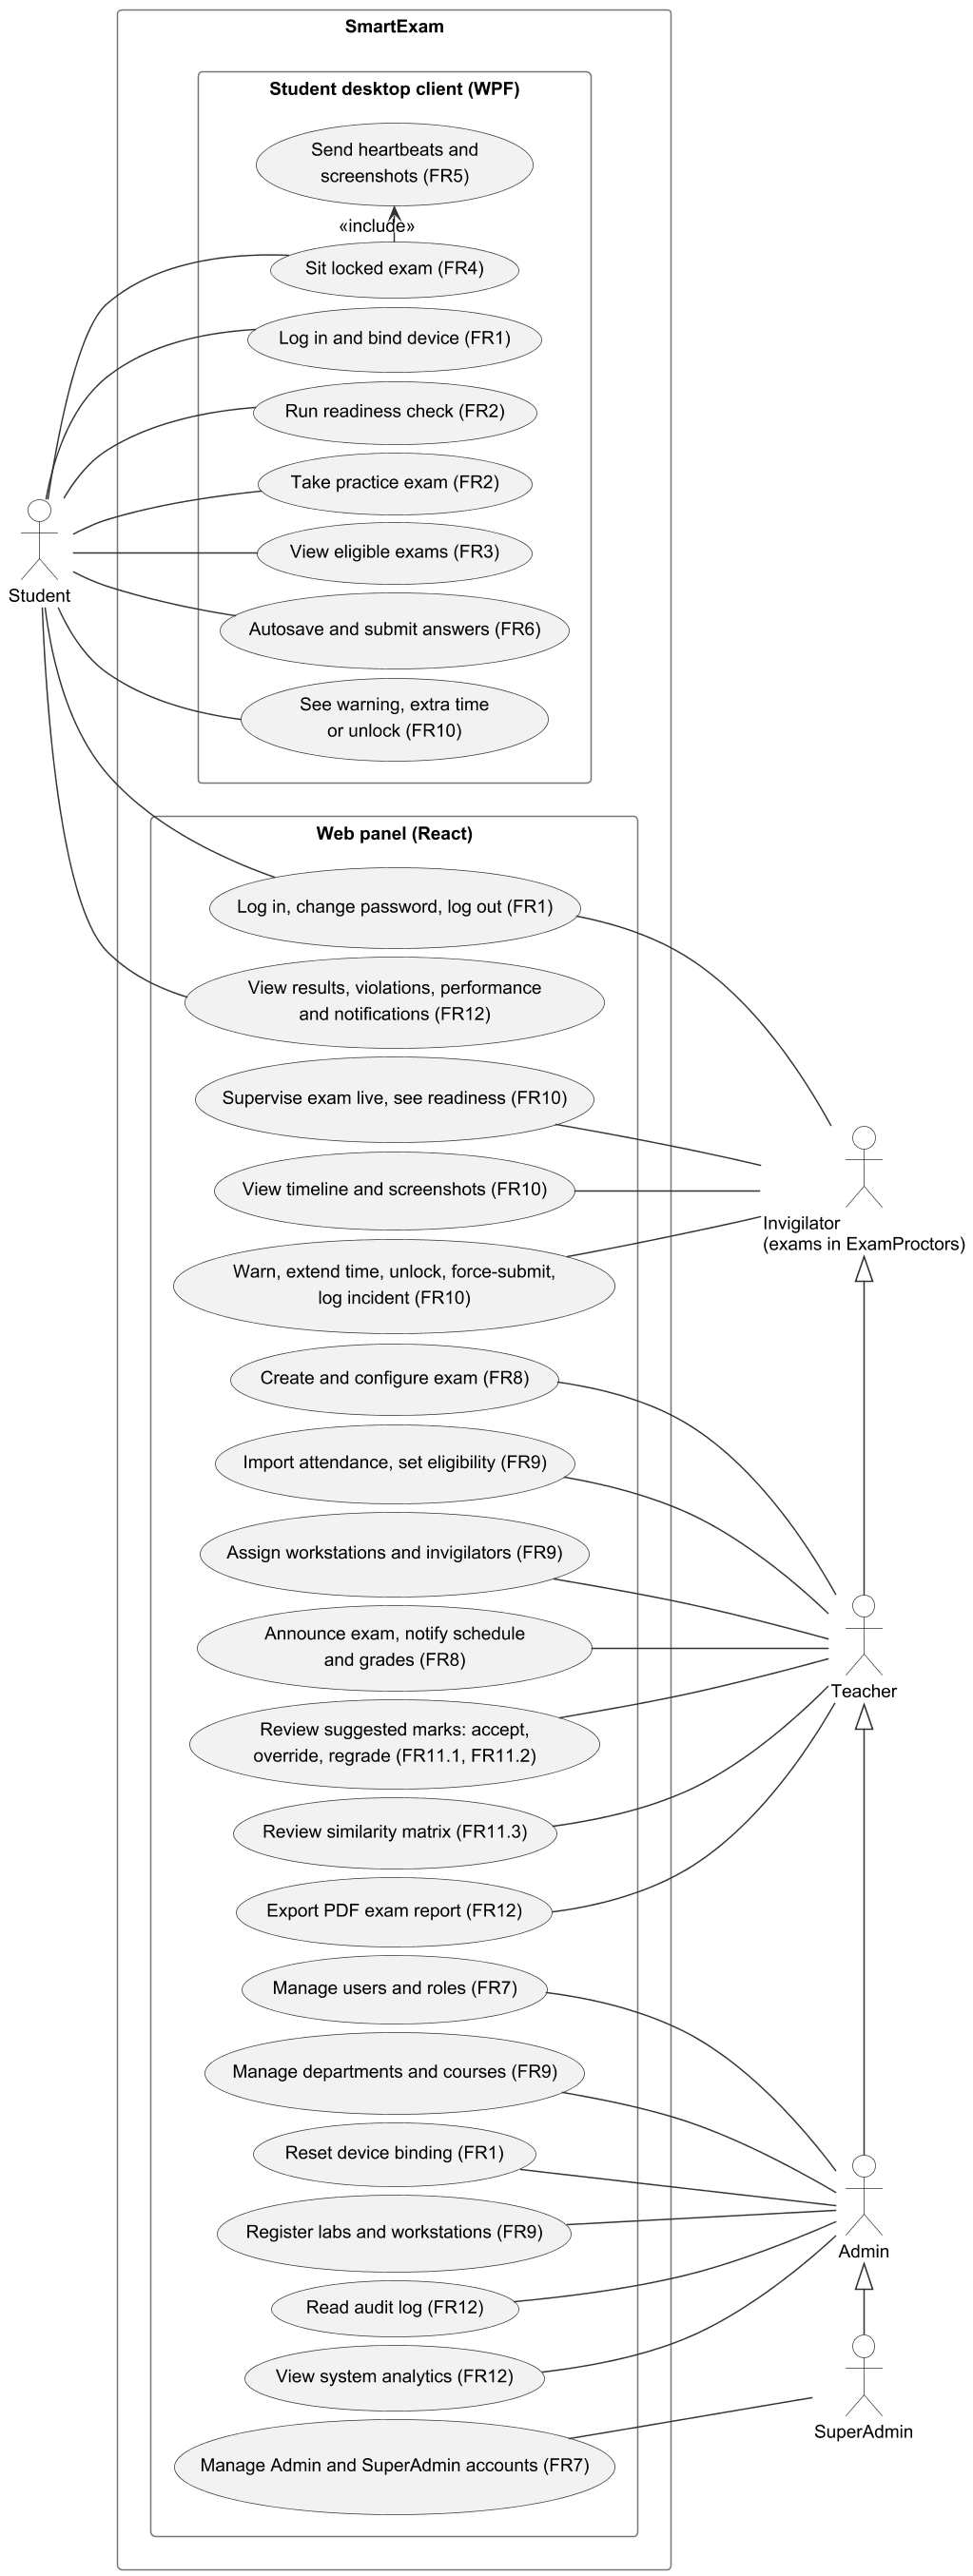
\includegraphics[height=0.86\textheight]{Figures/use_case_diagram.png}
\caption{Use Case Diagram of SmartExam}
\label{fig:usecase_diagram}
\end{figure}

\begin{sloppypar}
The API enforces this separation. Role attributes (\texttt{[Authorize(Roles=...)]}) restrict the endpoints, and \texttt{ExamAccessService} checks who may supervise a given exam.
\end{sloppypar}

\subsection{User Stories}

We wrote user stories to plan sprints and to define when a feature was done \cite{user_stories_applied}. Each story names the requirement it serves.

\subsubsection{Student}
\begin{enumerate}[nosep]
    \item As a student, I log in from the client and my account is bound to my lab PC, so nobody can sit my exam from another machine (FR1).
    \item As a student, I run a system check and an ungraded practice exam before the real one, so problems with my PC show up early (FR2).
    \item As a student, I see only the exams I am eligible for, with the start countdown and my check status (FR3).
    \item As a student, I sit the exam in a locked fullscreen window where only the allowed tools run, so every candidate works under the same rules (FR4).
    \item As a student, my answers are saved every 10 seconds and kept on the PC while the network is down, and I get a receipt hash when I submit (FR6).
    \item As a student, I see an invigilator's warning or extra time on my screen during the exam (FR10).
\end{enumerate}

\subsubsection{Teacher}
\begin{enumerate}[nosep,resume]
    \item As a teacher, I create an exam with MCQ, coding and theory questions, test cases, an allowed-apps list and a lockdown mode (FR8).
    \item As a teacher, I import attendance, override eligibility with a logged reason, and assign each student a workstation (FR9).
    \item As a teacher, I get screenshots at random 30--90~s intervals and on each violation, plus idle time and webcam status, as evidence (FR5).
    \item As a teacher, I watch live student tiles, open a student's timeline and screenshots, and warn, extend time or force-submit (FR10).
    \item As a teacher, coding answers are run against weighted test cases and theory answers get a suggested mark, which I can accept or override (FR11.1, FR11.2).
    \item As a teacher, I see a similarity matrix of submissions so that I can review likely copying myself (FR11.3).
    \item As a teacher, I export a PDF report of an exam's results (FR12).
\end{enumerate}

\subsubsection{Invigilator}
\begin{enumerate}[nosep,resume]
    \item As an invigilator, I see only the exams I am assigned to and can warn students, extend time and force a submission, but not grade (FR10).
\end{enumerate}

\subsubsection{Admin and SuperAdmin}
\begin{enumerate}[nosep,resume]
    \item As an admin, I create, import, deactivate and sign out users and assign their roles (FR7).
    \item As an admin, I reset a student's device binding when a lab PC is replaced (FR1).
    \item As an admin, I register labs and workstations with their PC names and IP addresses so that seats can be enforced (FR9).
    \item As an admin, I filter the audit log by event type to check logins, device bindings and eligibility overrides (FR12).
\end{enumerate}

\subsection{Use Case Descriptions}

Tables~\ref{tab:uct_auth_device} to~\ref{tab:uct_audit_report} describe the main use cases \cite{use_case_definition}; endpoint names are those of the backend.

\begin{table}[H]
\centering
\caption{UC-01: Log In and Verify Device Binding}
\label{tab:uct_auth_device}
{\small\renewcommand{\arraystretch}{1.15}
\begin{tabularx}{\textwidth}{>{\bfseries\raggedright\arraybackslash}p{2.3cm}>{\raggedright\arraybackslash}X}
\hline\hline
Actors & Student; \texttt{AuthController} \\
Pre-condition & Active student account; client running on a lab PC. \\
Main flow & 1.~Student enters email or roll number and password.\newline
2.~Client reads the BIOS, system-disk and baseboard serials through WMI and sends them with the PC name to \texttt{POST /api/auth/student-login}.\newline
3.~Server checks the PBKDF2 password hash and hashes the fingerprint with SHA-256.\newline
4.~If the account has no \texttt{DeviceBinding}, the hash is stored (audit \texttt{DEVICE\_BOUND}); otherwise it must match.\newline
5.~Server returns a JWT and a refresh token (audit \texttt{LOGIN\_SUCCESS}). \\
Exceptions & Wrong password: \texttt{LOGIN\_FAILED}. Inactive account: denied. Different PC: 401 \texttt{DEVICE\_MISMATCH}, logged; an admin must reset the binding. \\
Post-condition & Student is signed in on the bound PC. \\
\hline\hline
\end{tabularx}}
\end{table}

\begin{table}[H]
\centering
\caption{UC-02: Pass the Readiness Check and Start the Exam}
\label{tab:uct_pre_exam_check}
{\small\renewcommand{\arraystretch}{1.15}
\begin{tabularx}{\textwidth}{>{\bfseries\raggedright\arraybackslash}p{2.3cm}>{\raggedright\arraybackslash}X}
\hline\hline
Actors & Student; \texttt{ExamsController} \\
Pre-condition & Student is signed in and eligible for a scheduled exam (UC-01). \\
Main flow & 1.~Dashboard calls \texttt{GET /api/exams/student/current} for the exam, server time, check status and seat status.\newline
2.~Student runs the system check: API latency under 2~s, clock skew under 60~s, screen capture, webcam and microphone if the exam needs them, one monitor, no RDP or VM, keyboard hook, 200~MB free disk.\newline
3.~Client posts the result to \texttt{/api/exams/\{id\}/readiness}; the server recomputes the pass and stores a \texttt{ReadinessChecks} row.\newline
4.~Start unlocks at the opening time, measured on the server clock.\newline
5.~Student presses Start; the server checks eligibility, the seat, the exam window and, when the exam requires it, a passing check from the last 30 minutes, then creates an \texttt{ExamSession}. \\
Exceptions & Failed check: Retry, Start stays disabled. Server refusals: \texttt{READINESS\_REQUIRED}, \texttt{EXAM\_NOT\_STARTED}, \texttt{EXAM\_CLOSED}, or 403 \texttt{SEAT\_MISMATCH} (audited and shown on the live monitor). \\
Post-condition & Session is \texttt{InProgress}. \\
\hline\hline
\end{tabularx}}
\end{table}

\begin{table}[H]
\centering
\caption{UC-03: Sit the Locked Exam and Submit}
\label{tab:uct_lockdown_telemetry}
{\small\renewcommand{\arraystretch}{1.15}
\begin{tabularx}{\textwidth}{>{\bfseries\raggedright\arraybackslash}p{2.3cm}>{\raggedright\arraybackslash}X}
\hline\hline
Actors & Student; \texttt{MonitoringController}, \texttt{SubmissionService} \\
Pre-condition & Session is \texttt{InProgress} (UC-02). \\
Main flow & 1.~Exam window opens fullscreen and topmost; a low-level keyboard hook blocks Alt+Tab, the Windows key and Ctrl+Shift+Esc, and Task Manager is disabled.\newline
2.~Guards check processes every 2~s against the allowed apps (report or close, by lockdown mode) and watch the clipboard, USB, monitors, RDP and VMs.\newline
3.~Client sends a heartbeat every 10~s with focus, idle time and camera status; violations go in event batches with a screen capture; screenshots follow at random 30--90~s intervals.\newline
4.~Answers are autosaved every 10~s and written to an encrypted local backup.\newline
5.~Student submits; the server locks the session, returns a SHA-256 receipt, which the client checks, and queues the answers for grading. \\
Exceptions & Network loss: saves and events are queued and replayed later. Crash: answers are restored from the backup. Deadline: client auto-submits; the server times the session out 2 minutes after its end. \\
Post-condition & Session is \texttt{Submitted} or \texttt{TimedOut} with a stored receipt. \\
\hline\hline
\end{tabularx}}
\end{table}

\begin{table}[H]
\centering
\caption{UC-04: Configure an Exam and Its Access Rules}
\label{tab:uct_exam_config}
{\small\renewcommand{\arraystretch}{1.15}
\begin{tabularx}{\textwidth}{>{\bfseries\raggedright\arraybackslash}p{2.3cm}>{\raggedright\arraybackslash}X}
\hline\hline
Actors & Teacher (or Admin); \texttt{ExamsController} \\
Pre-condition & Teacher is signed in; the course section exists. \\
Main flow & 1.~Teacher enters title, start time, duration and instructions in the create-exam wizard.\newline
2.~Teacher adds MCQ, coding and theory questions with marks, test cases (public or hidden) and reference answers.\newline
3.~Teacher sets allowed apps, lockdown mode, readiness, webcam and microphone options, early join, minimum attendance and seat enforcement.\newline
4.~On the Eligibility page the teacher imports attendance (CSV), recalculates eligibility, overrides where needed and assigns workstations.\newline
5.~Teacher assigns invigilators to the exam. \\
Exceptions & Invalid fields are rejected. Bad CSV rows are reported per line. Recalculation after the exam has ended returns 409. \\
Post-condition & Exam is \texttt{Scheduled}; overrides are audited (\texttt{ELIGIBILITY\_OVERRIDDEN}). \\
\hline\hline
\end{tabularx}}
\end{table}

\begin{table}[H]
\centering
\caption{UC-05: Supervise a Live Exam}
\label{tab:uct_live_proctoring}
{\small\renewcommand{\arraystretch}{1.15}
\begin{tabularx}{\textwidth}{>{\bfseries\raggedright\arraybackslash}p{2.3cm}>{\raggedright\arraybackslash}X}
\hline\hline
Actors & Teacher or Invigilator; \texttt{MonitoringHub} (\texttt{/hubs/monitoring}) \\
Pre-condition & Exam is running; the staff member owns or is assigned to it. \\
Main flow & 1.~Staff member picks the exam on the Live Monitor; the page joins the exam's SignalR group.\newline
2.~Tiles update from \texttt{StudentHeartbeat}; events arrive as \texttt{ViolationEvent}, classed as Warning, Suspicious or Violation.\newline
3.~Staff member opens a student's drawer to see the event timeline and screenshots.\newline
4.~Staff member sends a warning (\texttt{SendWarning}), adds time (\texttt{ExtendStudentTime}), force-submits (\texttt{ForceSubmitSessionById}), unlocks the PC for up to 30 minutes (\texttt{UnlockSession}) or records an incident. \\
Exceptions & No heartbeat for 30~s: tile shows Disconnected until the student reconnects. Staff not assigned to the exam: the hub refuses the action. \\
Post-condition & Actions are stored and audited; the student sees the warning or new time. \\
\hline\hline
\end{tabularx}}
\end{table}

\begin{table}[H]
\centering
\caption{UC-06: Grade Submissions and Review Plagiarism}
\label{tab:uct_compilation_evaluation}
{\small\renewcommand{\arraystretch}{1.15}
\begin{tabularx}{\textwidth}{>{\bfseries\raggedright\arraybackslash}p{2.3cm}>{\raggedright\arraybackslash}X}
\hline\hline
Actors & Teacher; grading services \\
Pre-condition & Sessions are submitted, force-submitted or timed out. \\
Main flow & 1.~MCQ answers are marked by key.\newline
2.~C++ answers are compiled and run against each test case in a Docker \texttt{gcc:13} container; marks follow the weights of the passed cases.\newline
3.~Theory answers are compared with the reference answer by TF-IDF similarity, giving a suggested mark and a confidence (an external semantic grader is optional and off by default).\newline
4.~Answers in the exam are compared pairwise by k-gram winnowing; pairs above the threshold go to \texttt{PlagiarismResults} and the similarity matrix.\newline
5.~Teacher reviews the suggestions and the matrix and overrides marks where needed. \\
Exceptions & Compile error or time-out: the test case fails and the message is shown to the teacher. \\
Post-condition & Suggested marks in \texttt{AiGradingResults}; teacher changes in \texttt{TeacherGradeOverrides}. \\
\hline\hline
\end{tabularx}}
\end{table}

\begin{table}[H]
\centering
\caption{UC-07: Review the Audit Log and Export a Report}
\label{tab:uct_audit_report}
{\small\renewcommand{\arraystretch}{1.15}
\begin{tabularx}{\textwidth}{>{\bfseries\raggedright\arraybackslash}p{2.3cm}>{\raggedright\arraybackslash}X}
\hline\hline
Actors & Admin (audit log); Teacher or Admin (report) \\
Pre-condition & Exam has ended and marks are reviewed. \\
Main flow & 1.~Admin opens the audit log (\texttt{GET /api/audit-logs}), filtered by event type.\newline
2.~Teacher requests \texttt{POST /api/analytics/exams/\{id\}/report}.\newline
3.~QuestPDF builds a PDF with summary statistics, per-question performance and the score distribution.\newline
4.~The report is stored as an \texttt{ExamReports} row and downloaded. \\
Exceptions & Unknown exam: no report is generated. \\
Post-condition & Report file is available for download. \\
\hline\hline
\end{tabularx}}
\end{table}
